%% ใช้ XeLaTeX Compiler (ใน Overleaf เลือกที่ Menu)
% !TEX program = xelatex
\documentclass[11pt,a4paper]{article}

%% ---- LaTeX syntax utility package ---- %%
\usepackage{etoolbox}

%% ---- Set up paper margin ---- %%
\usepackage[a4paper,top=1in,bottom=1.25in,left=1.25in,right=1in]{geometry}

%% ---- Set up fonts and encoding ---- %%
\usepackage{fontspec}
\usepackage{xunicode}
\usepackage{xltxtra}
\usepackage{gensymb}
\usepackage{comment}


% Enable line breaks for Thai text
\XeTeXlinebreaklocale "th"
\XeTeXlinebreakskip = 0pt plus 2pt minus 1pt

% Set up Thai/Eng fonts
\newfontfamily{\thaifont}{Laksaman}[Scale=MatchLowercase]
\newfontfamily{\englishfont}{CMU Serif}[Scale=MatchLowercase]
\setmainfont{CMU Serif}
%
\usepackage[Latin, Thai]{ucharclasses}
\setTransitionTo{Thai}{\thaifont}
\setTransitionFrom{Thai}{\englishfont}

%% ---- Load line spacing package ---- %%
\usepackage{setspace}

% Introducing hair space 
\newrobustcmd{\hrsp}{\ifmmode\mskip1mu\else\kern0.0625em\fi}

%% ---- Set up hyperlinks and colors ---- %%
\usepackage{xcolor}
\usepackage[unicode=true]{hyperref}
\hypersetup{%
    colorlinks,%
    linkcolor={red!50!black},%
    citecolor={blue!50!black},%
    urlcolor={blue!80!black},%
}
\renewcommand\UrlFont{\normalfont}
%
\usepackage{physics} % สำหรับพิมพ์เครื่องหมายและสัญลักษณ์ในฟิสิกส์
\usepackage{booktabs}
\usepackage{siunitx} % สำหรับพิมพ์ปริมาณในหน่วย SI
\usepackage{lipsum}
\usepackage{amsmath}
\sisetup{unit-mode = text}% ทำให้พิมพ์สัญลักษณ์ micro และ degree ได้ถูกต้อง
%
\usepackage{tikz} % สำหรับวาด diagram
\usepackage{titling}
%
\newcommand{\subtitle}[1]{%
  \posttitle{%
    \par\end{center}
    \begin{center}\large#1\end{center}
    \vskip0.5em}%
}
\usepackage{multirow} %สำหรับ merge rows

%% ------- Document starts here ------- %%
\begin{document}
%เปลี่ยนเป็นศัพท์ภาษาไทย
\renewcommand{\tablename}{ตารางที่}
\renewcommand{\figurename}{รูปที่}


\title{Laboratory Report of Physics \\ 
	\textbf{Lab: Newton's rings}
}
\subtitle{SCPY294 Intermediate Physics Laboratory\\ Department of Physics, Faculty of Science, Mahidol University}
\author{
\textbf{Kritin Wiwatyothin}\\
\\
Teaching Assistant: Withheld for privacy
}

\date{
Experiment conducted: January 2026\\
Report submitted: February 2026
}

\maketitle
\hrule


%% --------------------------------------- %%

\section{บทนำ} \label{introduction}
การทดลองนี้เป็นการศึกษาปรากฏการณ์การแทรกสอดของคลื่นแสง (Interference) ผ่านอุปกรณ์ที่เรียกว่าวงแหวนนิวตัน (Newton's Rings) ซึ่งเกิดขึ้นเมื่อลำแสงตกกระทบผ่านเลนส์นูนที่มีรัศมีความโค้งมากซึ่งวางอยู่บนแผ่นแก้วราบ แสงจะเกิดการสะท้อนที่ผิวโค้งด้านล่างของเลนส์และผิวด้านบนของแผ่นแก้ว ก่อให้เกิดชั้นฟิล์มอากาศ (Air film) ที่มีความหนาแตกต่างกันไปตามแนวรัศมี ความต่างระยะทางเดินของแสงนี้ส่งผลให้เกิดการแทรกสอดทั้งแบบเสริมและหักล้างจนปรากฏเป็นแถบมืดและสว่างรูปวงกลม ข้อมูลที่ได้จากการวัดเส้นผ่านศูนย์กลางของวงแหวนเหล่านี้จะถูกนำมาวิเคราะห์เพื่อคำนวณหาค่าความยาวคลื่นของแสงจากหลอดโซเดียมต่อไป

\subsection*{วัตถุประสงค์} \label{objective}
\begin{enumerate}
    \item เพื่อศึกษาปรากฏการณ์แทรกสอดของคลื่นแสง
    \item เพื่ออาศัยปรากฏการณ์แทรกสอดในรูปแบบที่เรียกว่าวงแหวนนิวตันเพื่อหาค่าความยาวคลื่นแสงจากหลอดโซเดียม
\end{enumerate}

\subsection*{ทฤษฎี} \label{theory}

วงแหวนนิวตันเกิดขึ้นเมื่อแสงสีเดียว (Monochromatic Light) \cite{Hecht,Jenkins} ตกกระทบเลนส์นูนซึ่งวางอยู่บนแผ่นแก้วแบนราบ ทำให้เกิดการแทรกสอดกันระหว่างรังสีแสงที่สะท้อนจากผิวโค้งด้านล่างของเลนส์และรังสีแสงที่สะท้อนจากผิวด้านบนของแผ่นแก้วราบ โดยมีความต่างระยะทางเดินของแสง (Optical Path Difference) $\Delta l$ ในรูปทั่วไปคือ \cite{Hecht}
\begin{equation}
    \Delta l = 2\mu t \cos \theta  \label{eq:basic}
\end{equation} 
โดยที่ $\mu$ คือดัชนีหักเหของชั้นฟิล์มอากาศ ($\mu \approx 1$), $t$ คือความหนาของชั้นฟิล์มอากาศ ณ ตำแหน่งที่พิจารณา และ $\theta$ คือมุมหักเหภายในชั้นฟิล์ม

เนื่องจากการสะท้อนที่ผิวแก้วราบเป็นการสะท้อนจากตัวกลางที่มีดัชนีหักเหสูงกว่าอากาศ แสงจะมีการเปลี่ยนเฟสไป $\pi$ เรเดียน เงื่อนไขการแทรกสอดสำหรับแถบสว่าง (Bright Fringes) จึงเขียนได้เป็น
\begin{equation}
    2\mu t \cos \theta = \left(n + \frac{1}{2}\right)\lambda \label{eq:bright_condition}
\end{equation}
เมื่อ $n = 0, 1, 2, 3, \dots$ คือลำดับของวงแหวน และ $\lambda$ คือความยาวคลื่นแสงในสุญญากาศ

ในเชิงเรขาคณิต เมื่อพิจารณาเลนส์นูนรัศมีความโค้ง $R$ วางบนแผ่นแก้วราบ หากให้ $P$ คือรัศมีของวงแหวนที่วัดจากจุดสัมผัส ณ ตำแหน่งที่มีความหนาฟิล์มอากาศเป็น $t$ จากรูปเรขาคณิตจะได้ความสัมพันธ์ $R^2 = P^2 + (R-t)^2$ เมื่อกระจายพจน์จะได้:
\begin{align*}
    R^2 &= P^2 + R^2 - 2Rt + t^2 \\
    2Rt &= P^2 + t^2
\end{align*}
เนื่องจากความหนา $t$ มีค่าน้อยมากเมื่อเทียบกับรัศมีความโค้ง $R$ ($t \ll R$) ทำให้พจน์ $t^2$ มีค่าน้อยจนตัดทิ้งได้ จึงได้ความสัมพันธ์ระหว่างความหนาของฟิล์มอากาศและรัศมีวงแหวนเป็น
\begin{equation}
    t \approx \frac{P^2}{2R} \label{eq:geometry_t}
\end{equation}

เมื่อนำค่า $t$ จากสมการ (\ref{eq:geometry_t}) แทนลงในเงื่อนไขการแทรกสอดสำหรับแถบสว่างในสมการ (\ref{eq:bright_condition}) จะได้:
\begin{equation}
    2\mu \left( \frac{P^2}{2R} \right) \cos \theta = \left(n + \frac{1}{2}\right)\lambda \label{eq: medium}
\end{equation}
ในกรณีที่แสงตกกระทบผิวเลนส์ในแนวดิ่ง ($\theta \approx 0^\circ, \cos \theta \approx 1$) และตัวกลางเป็นอากาศ ($\mu = 1$) สมการจะลดรูปเป็น $P^2 / R = (n + 1/2)\lambda$ และเมื่อพิจารณาในรูปของเส้นผ่านศูนย์กลาง $D = 2P$ จะได้สมการสำหรับเส้นผ่านศูนย์กลางของวงแหวนสว่างดังนี้: \cite{Jenkins}
\begin{equation}
    D^2 = 4n\lambda R + 2\lambda R \label{eq:Diameter square}
\end{equation}






%% --------------------------------------- %%
\section{ขั้นตอนการทดลอง} \label{procedure}

\subsection*{ตอนที่ 1: การเตรียมอุปกรณ์และการตั้งค่าเริ่มต้น}
ในส่วนนี้มีวัตถุประสงค์เพื่อเตรียมชุดทดลองและปรับโฟกัสของกล้องจุลทรรศน์ให้พร้อมสำหรับการวัดขนาดวงแหวนนิวตัน โดยมีขั้นตอนดังนี้:
\begin{enumerate}
    \item ติดตั้งชุดทดลองโดยวางเลนส์นูนและแผ่นแก้วราบไว้บนฐานรองสีดำใต้กล้องจุลทรรศน์เวอร์เนียร์ดังรูปที่ \ref{Lab}
    \item จัดตำแหน่งของหลอดแสงโซเดียมให้ส่องสว่างเข้าหาแผ่นแก้วบางที่ทำมุมสะท้อนแสงลงสู่ชุดเลนส์
    \item ปรับแผ่นแก้วสะท้อนแสงเพื่อให้ลำแสงจากหลอดโซเดียมเข้าสู่ลำกล้องจุลทรรศน์ได้อย่างเต็มที่
    \item เลื่อนกล้องจุลทรรศน์ลงมาในตำแหน่งต่ำสุด แล้วค่อย ๆ ปรับโฟกัสขึ้นจนกระทั่งมองเห็นรูปแบบการแทรกสอดของวงแหวนนิวตันชัดเจนที่สุด
    \item ตรวจสอบให้แน่ใจว่าเห็นทั้งแถบสว่างและแถบมืดเรียงตัวเป็นวงกลมล้อมรอบจุดศูนย์กลาง
\end{enumerate}



\subsection*{ตอนที่ 2: การวัดขนาดเส้นผ่านศูนย์กลางของวงแหวน}
ในส่วนนี้มีวัตถุประสงค์เพื่อบันทึกตำแหน่งของวงแหวนสว่างเพื่อนำไปคำนวณหาเส้นผ่านศูนย์กลาง โดยมีขั้นตอนดังนี้:
\begin{enumerate}
    \item ปรับเลื่อนกล้องจุลทรรศน์เวอร์เนียร์ไปทางด้านซ้ายหรือขวาของจุดศูนย์กลาง เพื่อเลือกวงแหวนสว่างลำดับที่ต้องการเริ่มต้นวัด
    \item ใช้เครื่องหมายกากบาท (Crosshair) ในกล้องเล็งให้ตรงกับแถบสว่างของวงแหวนลำดับที่ $n$ จากนั้นบันทึกค่าตำแหน่งจากสเกลเวอร์เนียร์
    \item เลื่อนกล้องไปยังลำดับถัดไปและบันทึกค่าตำแหน่งของวงแหวนสว่างในทิศทางเดียวกันจนครบตามจำนวนที่กำหนด
    \item เลื่อนกล้องข้ามจุดศูนย์กลางไปยังวงแหวนฝั่งตรงข้าม และบันทึกตำแหน่งของวงแหวนสว่างในลำดับที่ตรงกัน
    \item คำนวณหาค่าเส้นผ่านศูนย์กลาง ($D$) ของวงแหวนแต่ละลำดับจากผลต่างของตำแหน่งฝั่งซ้ายและฝั่งขวา
\end{enumerate}

\subsubsection*{ตอนที่ 3: การหารัศมีความโค้งของเลนส์นูนแกมระนาบ}
\begin{enumerate}
    \item นำเลนส์นูนแกมระนาบที่ใช้ในการทดลองมาวัดค่าความสูงของส่วนโค้ง ($h$) ด้วย สเฟียโรมิเตอร์ (Spherometer)
    \item ทำการวัดค่าระยะห่างระหว่างขาของสเฟียโรมิเตอร์โดยเฉลี่ย ($a$) และบันทึกค่าเพื่อนำไปคำนวณหารัศมีความโค้ง $R$ จากสมการ:
    \begin{equation}
    R = \frac{a^2}{6h} + \frac{h}{2}
    \end{equation}
    \item ทำการวัดซ้ำเพื่อหาค่าเฉลี่ยและค่าความคลาดเคลื่อน ($\Delta R$) เพื่อใช้เป็นตัวแปรคงที่ในการคำนวณหาค่าความยาวคลื่นแสงต่อไป
\end{enumerate}

\subsection*{ตอนที่ 4: การวิเคราะห์ข้อมูลเพื่อหาความยาวคลื่น}
ในส่วนนี้มีวัตถุประสงค์เพื่อนำข้อมูลที่วัดได้มาวิเคราะห์หาค่าความยาวคลื่นของแสงโซเดียม โดยมีขั้นตอนดังนี้:
\begin{enumerate}
    \item นำค่าเส้นผ่านศูนย์กลางที่ได้มาคำนวณเป็นค่า $D^2$ สำหรับวงแหวนสว่างแต่ละลำดับ $n$
    \item สร้างกราฟความสัมพันธ์ระหว่างค่า $D^2$ กับลำดับของวงแหวน $n$ เพื่อตรวจสอบความเป็นเส้นตรง
    \item หาค่าความชัน ($m$) ของกราฟโดยใช้วิธีการวิเคราะห์ข้อมูลแบบ Curve Fitting จากสมการที่ \ref{eq:Diameter square}
    โดยที่ความชัน $m = 4\lambda R$ และจุดตัดแกน $y$ คือ $2\lambda R$
    \item คำนวณหาค่าความยาวคลื่น $\lambda$ ของหลอดแสงโซเดียมได้จากค่าความชัน โดยใช้รัศมีความโค้งของเลนส์ $R$ ที่วัดมาได้ และเปรียบเทียบกับค่ามาตรฐานที่ $589.0$ nm \cite{Sodium}
\end{enumerate}

\begin{figure}[htbp]
    \centering
    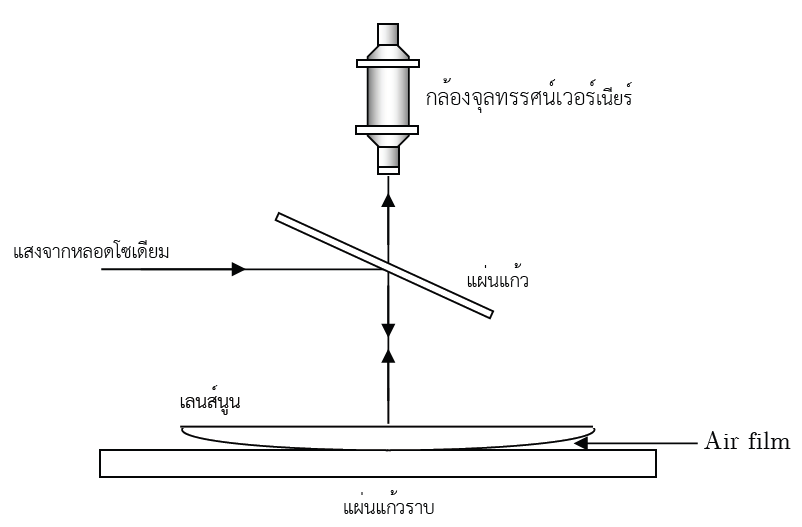
\includegraphics[width=0.9\textwidth]{ชุดการทดลอง.png}
    \caption{ชุดการทดลองวงแหวนนิวตัน}
    \label{Lab}
\end{figure}

\begin{figure}[htbp]
    \centering
    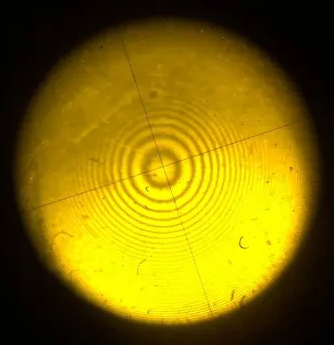
\includegraphics[width=0.3\textwidth]{NewtonRing.png}
    \caption{ตัวอย่าง Newton's Ring}
    \label{Lab}
\end{figure}


%% --------------------------------------- %%
\newpage
\section{ผลการทดลอง} \label{result}

\subsection{ข้อมูลจากการทดลอง} \label{data}
ภายในการทดลองมีการวัดค่าระยะห่างระหว่างขาของสเฟียโรมิเตอร์ได้เป็น $4.00 \, \text{cm}$, $4.10 \, \text{cm}$, และ $4.15 \, \text{cm}$ ซึ่งมีค่าคาดเคลื่อนจากสเกลเป็น $0.01$ cm และเมื่อนำมาหาค่าเฉลี่ยจะได้ $a = 4.08 \pm 0.02 \, \text{cm}$ นอกจากนี้ยังค่าความสูงส่วนโค้งที่วัดได้คือ $h = 0.54 \pm 0.01\,\text{cm}$ จึงนำมาวัดเป็นค่ารัศมีความโค้งได้เป็น $R = 51 \pm 1 \, \text{cm}$
โดยจากการทดลองได้ตารางข้อมูลดังนี้

\begin{table}[htbp]
\centering
\caption{บันทึกค่าตำแหน่งจากการวัดวงแหวนนิวตันฝั่งซ้าย ($r_1$) และฝั่งขวา ($r_2$)}
\renewcommand{\arraystretch}{1.2}
\begin{tabular}{|c|ccc|c|ccc|c|c|}
\hline
\multirow{2}{*}{$n$} 
& \multicolumn{3}{c|}{$r_1$ ($\pm 0.001$ cm)} 
& \multirow{2}{*}{$\bar{r_1}$  (cm)}
& \multicolumn{3}{c|}{$r_2$ ($\pm 0.001$ cm)} 
& \multirow{2}{*}{$\bar{r_2}$ (cm)}
& \multirow{2}{*}{$D$ (mm)} \\
\cline{2-4} \cline{6-8}
& ครั้งที่ 1 & ครั้งที่ 2 & ครั้งที่ 3 & & ครั้งที่ 1 & ครั้งที่ 2 & ครั้งที่ 3 & & \\
\hline
0 & 7.052 & 7.055 & 7.057 & 7.05 $\pm$ 0.04 & 7.005 & 7.006 & 7.005 & 7.01 $\pm$ 0.02 & 0.05 $\pm$ 0.04 \\
1 & 7.081 & 7.088 & 7.085 & 7.08 $\pm$ 0.05 & 6.965 & 6.969 & 6.968 & 6.97 $\pm$ 0.03 & 0.12 $\pm$ 0.06 \\
2 & 7.104 & 7.108 & 7.105 & 7.11 $\pm$ 0.03 & 6.952 & 6.948 & 6.947 & 6.95 $\pm$ 0.04 & 0.16 $\pm$ 0.05 \\
3 & 7.118 & 7.121 & 7.120 & 7.12 $\pm$ 0.03 & 6.932 & 6.930 & 6.931 & 6.93 $\pm$ 0.02 & 0.19 $\pm$ 0.04 \\
4 & 7.134 & 7.135 & 7.136 & 7.14 $\pm$ 0.02 & 6.920 & 6.918 & 6.920 & 6.92 $\pm$ 0.03 & 0.22 $\pm$ 0.04 \\
5 & 7.145 & 7.146 & 7.147 & 7.15 $\pm$ 0.02 & 6.905 & 6.906 & 6.909 & 6.91 $\pm$ 0.03 & 0.24 $\pm$ 0.04 \\
6 & 7.156 & 7.153 & 7.154 & 7.15 $\pm$ 0.03 & 6.897 & 6.898 & 6.893 & 6.90 $\pm$ 0.04 & 0.26 $\pm$ 0.05 \\
7 & 7.167 & 7.167 & 7.165 & 7.17 $\pm$ 0.03 & 6.890 & 6.891 & 6.888 & 6.89 $\pm$ 0.03 & 0.28 $\pm$ 0.04 \\
\hline
\end{tabular}
\end{table}


\begin{table}[htbp]
\centering
\caption{ผลการคำนวณค่าเส้นผ่านศูนย์กลางยกกำลังสอง ($D^2$) สำหรับการวิเคราะห์กราฟ}
\renewcommand{\arraystretch}{1.2}
\begin{tabular}{|c|c|c|}
\hline
ลำดับวงที่ ($n$) & $D$ (cm) & $D^2$ ($\text{cm}^2$) \\
\hline
0 & 0.05 $\pm$ 0.04 & 0.002 $\pm$ 0.002 \\
1 & 0.12 $\pm$ 0.06 & 0.014 $\pm$ 0.003 \\
2 & 0.16 $\pm$ 0.05 & 0.025 $\pm$ 0.003 \\
3 & 0.19 $\pm$ 0.04 & 0.036 $\pm$ 0.001 \\
4 & 0.22 $\pm$ 0.04 & 0.047 $\pm$ 0.001 \\
5 & 0.24 $\pm$ 0.04 & 0.057 $\pm$ 0.002 \\
6 & 0.26 $\pm$ 0.05 & 0.067 $\pm$ 0.002 \\
7 & 0.28 $\pm$ 0.04 & 0.077 $\pm$ 0.002 \\
\hline
\end{tabular}
\end{table}




\newpage
\subsection{การคำนวณความคลาดเคลื่อน}

ค่าความคลาดเคลื่อนที่เกิดขึ้นในการทดลองนี้มีแหล่งที่มาหลักจากการอ่านตำแหน่งของวงแหวน และการวัดพารามิเตอร์ทางกายภาพของเลนส์ด้วยสเฟียโรมิเตอร์ ซึ่งสามารถแบ่งแหล่งที่มาได้ดังนี้

\subsubsection{ความคลาดเคลื่อนของตำแหน่งวงแหวน $r_1$ และ $r_2$}

ในการวัดตำแหน่งของวงแหวนแต่ละข้าง ($r_1$ และ $r_2$) มีความคลาดเคลื่อนจากสเกลเวอร์เนียร์ของกล้องจุลทรรศน์ที่มีความละเอียดต่ำสุด $0.001\ \text{cm}$ จึงกำหนดให้ความคลาดเคลื่อนเชิงระบบเป็น $\delta_{sys} = 0.001\ \text{cm}$ 

เนื่องจากการทดลองมีการวัดซ้ำในแต่ละลำดับ $3$ ครั้ง ความคลาดเคลื่อนเชิงสถิติ (statistical error) จึงคำนวณจากค่าเบี่ยงเบนมาตรฐานของค่าเฉลี่ย (Standard Error of the Mean) ดังนี้
\[
\delta_{r_{stat}} = \frac{1}{\sqrt{N}} \sqrt{\frac{1}{N-1}\sum_{i=1}^{N}(r_i-\bar{r})^2}
\]
โดยค่าความคลาดเคลื่อนรวมของตำแหน่งเฉลี่ย ($\delta \bar{r}$) คำนวณได้จาก $\delta \bar{r} = \sqrt{\delta_{stat}^2 + \delta_{sys}^2}$

\subsubsection{ความคลาดเคลื่อนของเส้นผ่านศูนย์กลาง $D$ และ $D^2$}

เส้นผ่านศูนย์กลาง $D = |\bar{r}_1 - \bar{r}_2|$ มีความคลาดเคลื่อนเป็น $\delta D = \sqrt{(\delta \bar{r}_1)^2 + (\delta \bar{r}_2)^2}$ และสำหรับการนำค่า $D$ ไปยกกำลังสอง ความคลาดเคลื่อน $\delta D^2$ คำนวณได้จาก
\[
\delta D^2 = \left| \frac{d(D^2)}{dD} \right| \delta D = 2D \cdot \delta D
\]

\subsubsection{ความคลาดเคลื่อนของรัศมีความโค้งเลนส์ $R$ จากสเฟียโรมิเตอร์}



เนื่องจากรัศมีความโค้ง $R$ คำนวณจากระยะห่างระหว่างขา ($a$) และความสูงส่วนโค้ง ($h$) ตามสมการ $R = \frac{a^2}{6h} + \frac{h}{2}$ ความคลาดเคลื่อน $\delta R$ จึงต้องพิจารณาการส่งผ่านความคลาดเคลื่อนจากทั้งสองตัวแปรดังนี้
\[
\delta R = \sqrt{ \left( \frac{\partial R}{\partial a} \delta a \right)^2 + \left( \frac{\partial R}{\partial h} \delta h \right)^2 } = \sqrt{ \left( \frac{a}{3h} \delta a \right)^2 + \left( \left( -\frac{a^2}{6h^2} + \frac{1}{2} \right) \delta h \right)^2 }
\]
โดยที่ $\delta a$ และ $\delta h$ คือความคลาดเคลื่อนรวม (Combined Uncertainty) ที่ได้จากการวัดซ้ำและการอ่านค่าจากสเกลของสเฟียโรมิเตอร์

\subsubsection{ความคลาดเคลื่อนของความยาวคลื่นแสง $\lambda$}

ความยาวคลื่นแสงคำนวณจากความชันของกราฟ ($m$) ตามความสัมพันธ์ $\lambda = m / (4R)$ ดังนั้นความคลาดเคลื่อนสัมพัทธ์ของ $\lambda$ จะพิจารณาจากความคลาดเคลื่อนของความชัน ($\delta m$) ที่ได้จากการทำ Least squares fitting \cite{Taylor} และความคลาดเคลื่อนของรัศมีความโค้ง ($\delta R$) ที่คำนวณได้จากหัวข้อก่อนหน้า
\[
\frac{\delta \lambda}{\lambda} = \sqrt{ \left( \frac{\delta m}{m} \right)^2 + \left( \frac{\delta R}{R} \right)^2 }
\]





%% -------------------------------------------- %%

\subsection{การวิเคราะห์ผลและอภิปรายผล} \label{analysis}

\subsection*{การหาค่าความยาวคลื่นแสงจากผลการทดลอง}

จากผลการทดลองและการวัดขนาดของวงแหวนนิวตัน เราได้ชุดข้อมูลความสัมพันธ์ระหว่างลำดับของวงแหวน ($n$) และเส้นผ่านศูนย์กลางยกกำลังสอง ($D^2$) ซึ่งความสัมพันธ์ดังกล่าวเป็นไปตามทฤษฎีการแทรกสอดของแสงผ่านฟิล์มบางอากาศตามสมการที่ (\ref{eq:Diameter square}) โดยจุดตัดแกนจึงถูกพิจารณาเป็นค่าคงที่ $c$ และความชันของกราฟ $m = 4\lambda R$ ได้เป็นดังสมการต่อไปนี้
\begin{equation}
D^2 = mn + c
\end{equation}
โดยที่ $\lambda$ คือค่าความยาวคลื่นของแสงโซเดียมที่ต้องการทราบค่า, $R$ คือรัศมีความโค้งของเลนส์นูน และ $c$ คือค่าคงที่ซึ่งเป็นจุดตัดแกน $y$ ที่สะท้อนถึงระยะห่างระหว่างเลนส์และแผ่นแก้วราบ ณ จุดสัมผัส (Phase shift หรือความไม่สะอาดที่จุดสัมผัส)

\textbf{\underline{หมายเหตุ}} สาเหตุที่กำหนดให้ $c$ เป็นพารามิเตอร์อิสระนั้น เพราะมันช่วยให้การคำนวณค่าความยาวคลื่นจากความชันของกราฟมีความถูกต้องและลดอิทธิพลจาก Systematic Error ได้ดีกว่าการทำ Curve Fitting ไปพร้อมกับ \mbox{ค่าความชัน}

\newpage

\subsection*{กราฟแสดงความสัมพันธ์ระหว่าง $D^2$ และลำดับวงแหวน} \label{graph}

\pagestyle{plain}
จากการทำการฟิตกราฟโดยใช้โปรแกรม \texttt{Python} (Library: \texttt{lmfit}) \cite{LMFIT} กับสมการเชิงเส้นข้างต้น จะได้กราฟดังรูปที่ \ref{fig:graph1} ซึ่งแสดงความสัมพันธ์ของวงแหวนนิวตันที่วัดได้ และได้ผลลัพธ์พารามิเตอร์ที่สำคัญดังนี้

\begin{figure}[h]
	\centering
	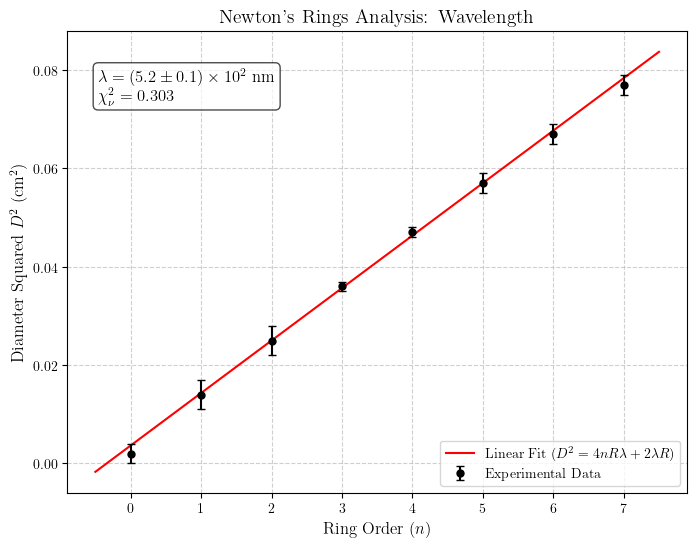
\includegraphics[width=0.85\textwidth]{GraphRing.png}
	\caption{กราฟแสดงความสัมพันธ์ระหว่างเส้นผ่านศูนย์กลางยกกำลังสอง $D^2$ กับลำดับของวงแหวน $n$}
    \label{fig:graph1}
\end{figure}



\bigskip

\begin{itemize}

    \item Chi-square (Reduced): $\chi_{\nu}^2 = 0.3026$
    \medskip
    \item ค่าความยาวคลื่นแสงโซเดียม $\lambda$ ที่คำนวณได้ : $\lambda = (5.2 \pm 0.1) \times 10^2 \ \text{nm}$
    \medskip
    \item ค่าความยาวคลื่นแสงโซเดียม $\lambda$ ที่ปรับแล้ว (หารด้วย $\sqrt{\chi_{\nu}^2}$): \mbox{$\lambda = (520 \pm 30)\ \text{nm}$}
    \item จุดตัดแกน $y$ ที่คำนวณได้และปรับแล้ว (หารด้วย $\sqrt{\chi_{\nu}^2}$): $c = 0.004 \pm 0.001 \ \text{cm}^2$
    \medskip

\end{itemize}

\textbf{\underline{หมายเหตุ}} ค่าความคลาดเคลื่อนของความยาวคลื่นแสงที่คำนวณได้โดยไม่ปรับเลขนัยสำคัญคือ $14$ nm

จุดตัดแกน $y$ ($c$) ที่ได้จากการ Fit มีค่าเท่ากับ $0.004 \pm 0.001\ \text{cm}^2$ ซึ่งมีความแตกต่างจากค่าทางทฤษฎี ($2\lambda R$) สาเหตุอาจเนื่องมาจากความไม่สมบูรณ์ของผิวสัมผัสระหว่างเลนส์และแผ่นแก้วราบ หรือความคลาดเคลื่อนในการเล็งตำแหน่งวงแหวน


\newpage
\section*{อภิปรายผล}

จากการทดลองนี้ ได้ทำการศึกษาความสัมพันธ์ระหว่างเส้นผ่านศูนย์กลางยกกำลังสองของวงแหวนนิวตัน $D^2$ และลำดับของวงแหวนสว่าง $n$ เพื่อหาค่าความยาวคลื่นของแสงโซเดียม โดยใช้เลนส์นูนที่มีรัศมีความโค้ง $R = 51 \pm 1$ cm 

เมื่อพล็อตกราฟ $D^2$ กับ $n$ และทำการฟิตด้วยสมการเชิงเส้น
\[
D^2 = 4nR\lambda + c
\]
พบว่าข้อมูลมีความสัมพันธ์เชิงเส้นที่ชัดเจน ซึ่งสอดคล้องกับทฤษฎีการแทรกสอดของแสงผ่านฟิล์มบางอากาศ (Newton's Rings) โดยค่าความยาวคลื่น $\lambda$ สามารถหาได้จากความชันของกราฟ $m = 4R\lambda$
\newline
\medskip

\textbf{ผลการวิเคราะห์ทางสถิติ} การฟิตกราฟให้ค่าความยาวคลื่น
\[
\lambda = (520 \pm 14)\ \text{nm}
\]
และมีค่า reduced chi-square เท่ากับ
\[
\chi_{\nu}^2 = 0.3026
\]
ซึ่งมีค่าน้อยกว่าหนึ่ง แสดงว่าความไม่แน่นอนของข้อมูลที่ประเมินจากการอ่านค่าตำแหน่งวงแหวนอาจถูกประเมินไว้สูงเกินจริง และเมื่อทำการปรับค่าความไม่แน่นอนโดยหารด้วย $\sqrt{\chi_{\nu}^2}$ จะได้ค่าที่ปรับแล้วเป็น
\[
\lambda = (5.2 \pm 0.3) \times 10^2\ \text{nm}
\]

\newline
\medskip



\textbf{การวิเคราะห์จุดตัดแกนและความไม่สอดคล้องทางทฤษฎี:} 
จากการพิจารณาผลการฟิตกราฟ พบว่าจุดตัดแกน y มีค่าเท่ากับ
\[
c = 0.004 \pm 0.001\ \text{cm}^2 
\]
ซึ่งหากพิจารณาตามทฤษฎีที่ระบุว่า $c = 2\lambda R$ จะพบว่าค่าที่ได้จากการฟิตนี้มีความไม่สอดคล้องกับค่า $\lambda$ ที่คำนวณได้จากความชัน 



ความแตกต่างดังกล่าวสะท้อนให้เห็นถึงความไม่อุดมคติของระบบทดลอง (Systematic Error) อาทิ การที่ผิวสัมผัสระหว่างเลนส์และแผ่นแก้วราบไม่ได้สัมผัสกันสนิท 100\% ณ จุดกำเนิด ($n=0$) ซึ่งส่งผลให้ระยะห่างฟิล์มอากาศเริ่มต้นมีค่ามากกว่าทฤษฎี การที่เราเลือกกำหนดให้ $c$ เป็นพารามิเตอร์อิสระแทนการบังคับให้เป็นไปตามเงื่อนไข $2\lambda R$ จึงมีความเหมาะสมกว่าในเชิงการวิเคราะห์ข้อมูล เพราะช่วยป้องกันไม่ให้ความคลาดเคลื่อนที่จุดสัมผัสนั้นไปส่งผลบิดเบือนต่อค่าความชันของกราฟ ทำให้ค่าความยาวคลื่น $\lambda$ ที่ได้จากความชันยังคงมีความถูกต้องและสะท้อนพฤติกรรมการเปลี่ยนลำดับวงแหวนได้อย่างแม่นยำที่สุดเท่าที่จะเป็นไปได้ในขอบเขตของการทดลอง

\newline
\medskip

โดยรวมแล้ว การทดลองนี้สามารถแสดงให้เห็นปรากฏการณ์การแทรกสอดและสามารถคำนวณหาค่าความยาวคลื่นแสงได้ใกล้เคียงกับค่ามาตรฐาน (Sodium $D$-line $\approx 589$ nm) แม้จะมีความคลาดเคลื่อนร้อยละประมาณ $11.7\%$ ซึ่งสาเหตุหลักอาจมาจากความละเอียดของกล้องจุลทรรศน์ที่ใช้เล็งตำแหน่งวงแหวน ความคลาดเคลื่อนในการวัดจากผู้ทดลอง และรัศมีความโค้งของเลนส์ $R$ ที่ใช้ในการคำนวณอาจมีความแตกต่างจากค่าที่ระบุไว้เล็กน้อย



\newpage
\section{สรุป} \label{conclusion}

การทดลองนี้ได้ศึกษาปรากฏการณ์การแทรกสอดของแสงผ่านฟิล์มบางอากาศในลักษณะของวงแหวนนิวตัน เพื่อคำนวณหาค่าความยาวคลื่นของแสงโซเดียม โดยวัดเส้นผ่านศูนย์กลางของวงแหวนลำดับต่าง ๆ ด้วยกล้องจุลทรรศน์ และวิเคราะห์ความสัมพันธ์ระหว่างเส้นผ่านศูนย์กลางยกกำลังสอง ($D^2$) กับลำดับของวงแหวน ($n$) ด้วยการฟิตกราฟเชิงเส้น



ค่าความยาวคลื่นของแสงโซเดียมที่ได้จากการทดลอง (พร้อมค่าความคลาดเคลื่อนที่ปรับแล้ว) สรุปได้ดังนี้

\begin{align*}
\lambda &= (5.2 \pm 0.3) \times 10^2 \ \text{nm} \\
\end{align*}
ผลการทดลองแสดงให้เห็นความสัมพันธ์เชิงเส้นระหว่าง $D^2$ และ $n$ อย่างชัดเจน ซึ่งสอดคล้องกับทฤษฎีการแทรกสอด แม้ค่าความยาวคลื่นที่คำนวณได้จะมีความคลาดเคลื่อนจากค่ามาตรฐาน (589.0 nm) อยู่ประมาณ 11.7\% แต่ค่าที่ได้ยังคงอยู่ในขอบเขตของการทดลอง และค่า Reduced chi-square ที่ต่ำแสดงถึงความสอดคล้องที่ดีระหว่างข้อมูลกับโมเดล สรุปได้ว่าการทดลองนี้สามารถอธิบายพฤติกรรมการแทรกสอดของแสงและใช้ในการหาค่าความยาวคลื่นได้ถูกต้องภายใต้ขอบเขตความละเอียดของอุปกรณ์วัด

\newpage
\section*{คำถามท้ายการทดลอง}

\begin{enumerate}
    \item \textbf{จงแสดงที่มาของสมการที่ (\ref{eq:basic})} 
    
    \textbf{ตอบ:} สมการที่ (\ref{eq:basic}) $\Delta l = 2\mu t \cos\theta$ คือความต่างของเส้นทางเดินแสงพิจารณาได้จากทางเดินแสงในฟิล์มบางได้ดังนี้:
    \begin{itemize}
        \item จากความสัมพันธ์ของผลต่างเส้นทางเดินแสงเชิงแสง: $\Delta l = 2\mu PC - \mu_0 P_1A$
        \item โดยที่ $P_1A = PP_1 \sin\alpha$ และจากกฎของสเนลล์ $\mu_0 \sin\alpha = \mu \sin\theta$ จะได้ 
        \[\Delta l = 2\mu PC - \mu PP_1 \sin\theta\]
        \item จาก Geometry ของชั้นฟิล์มที่มีความหนา $t$ จะได้ระยะ $PC = \frac{t}{\cos\theta}$ และ $PP_1 = 2t \tan\theta$
        \item เมื่อแทนค่าลงในสมการจะได้:
        \[ \Delta l = 2\mu \left( \frac{t}{\cos\theta} \right) - \mu (2t \tan\theta) \sin\theta = 2\mu t \left( \frac{1 - \sin^2\theta}{\cos\theta} \right) \]
        \item \mbox{โดยใช้เอกลักษณ์ทางตรีโกณมิติ $1 - \sin^2\theta = \cos^2\theta$ จะได้ผลลัพธ์คือ $\Delta l = 2\mu t \cos\theta$ ตามสมการที่ (\ref{eq:basic})}
    \end{itemize}

    \item \textbf{ถ้าเปลี่ยนแปลงตัวกลางระหว่างเลนส์นูนกับแผ่นแก้วราบจะเกิดผลอย่างไรต่อขนาดของวงแหวนนิวตัน}
    
    \textbf{ตอบ:} หากเปลี่ยนตัวกลางจากอากาศเป็นของเหลวที่มีดัชนีหักเห $\mu$ สูงขึ้น ขนาดของวงแหวนนิวตันจะเล็กลง เนื่องจากรัศมีของวงแหวน ($P$) มีความสัมพันธ์ผกผันกับดัชนีหักเหของตัวกลางตามสมการ $P^2 = \frac{\lambda R (n+\frac{1}{2})}{\mu \cos\theta}$ ตามสมการที่ \ref{eq: medium} ส่งผลให้ความยาวคลื่นเชิงแสงในตัวกลางลดลง ($\lambda_n = \lambda / \mu$) ตำแหน่งของการแทรกสอดแต่ละลำดับจึงขยับเข้าใกล้จุดศูนย์กลางมากขึ้น

    \item \textbf{ความรู้เรื่องวงแหวนนิวตันสามารถนำไปประยุกต์ใช้ในเรื่องใด}
    
    \textbf{ตอบ:} ปรากฏการณ์วงแหวนนิวตันสามารถนำไปประยุกต์ใช้ได้หลากหลายสถานการณ์ เช่น:
    \begin{itemize}
        \item \textbf{การหาค่าความยาวคลื่นของแสง ($\lambda$):} ใช้ระบุค่าความยาวคลื่นของแหล่งกำเนิดแสงสีเดียวโดยอาศัยการวัดขนาดวงแหวน
        \item \textbf{การทดสอบคุณภาพผิวสัมผัส:} ใช้ตรวจสอบความราบเรียบหรือความโค้งที่สม่ำเสมอของผิวเลนส์ หากวงแหวนบิดเบี้ยวแสดงว่าผิวสัมผัสมีความขรุขระหรือไม่เป็นทรงกลมที่สมบูรณ์
        \item \textbf{การวัดดัชนีหักเหของของเหลว:} โดยการนำของเหลวไปแทนที่ช่องว่างอากาศแล้วสังเกตการเปลี่ยนแปลงรัศมีของวงแหวน
    \end{itemize}
\end{enumerate}



%%----------------------------------------%%
\newpage
\begin{thebibliography}{9}

\bibitem{Hecht}
Eugene Hecht,
\textit{Optics},
5th Edition,
Pearson Education, 2017.

\bibitem{Halliday}
David Halliday, Robert Resnick, and Jearl Walker,
\textit{Fundamentals of Physics},
10th Edition,
Wiley, 2013.

\bibitem{Jenkins}
Francis A. Jenkins and Harvey E. White,
\textit{Fundamentals of Optics},
4th Edition,
McGraw-Hill, 1981.

\bibitem{Taylor}
John R. Taylor,
\textit{An Introduction to Error Analysis: The Study of Uncertainties in Physical Measurements},
2nd Edition,
University Science Books, 1997.

\bibitem{LMFIT}
Matthew Newville et al.,
“LMFIT: Non-Linear Least-Square Minimization and Curve-Fitting for Python,”
Available: \url{https://lmfit.github.io/lmfit-py/}

\bibitem{Sodium}
National Institute of Standards and Technology (NIST),
“Sodium Spectral Lines,”
Available: \url{https://physics.nist.gov}

\end{thebibliography}
\end{document}
%